% Apéndice Campos Magnéticos Superficiales

\chapter{Campos Magnéticos Superficiales} % Main appendix title

\label{AppendixCamposMagneticosSuperficiales} % For referencing this appendix elsewhere, use \ref{AppendixA}

Los campos magnéticos próximos a las superficies de separación entre medios experimentan una suave transición entre las condiciones de frontera  y los campos impuestos macroscópicamente por la magnetización dominante en volumen. En particular nos interesarán los campos en el aire cercanos a las superficies de sólidos que puedan tener o no corrientes superficiales.


\section{Frontera magnética.}

El campo magnético exterior próximo a la superficie de los sólidos es afectado tanto por las condiciones de frontera entre el medio y el sólido como por la presencia de anomalías en el seno de material. Las dos propiedades más relevantes serán $\mu$ y $\sigma_{e}$ (la permeabilidad magnética y la conductividad eléctrica) las que nos permitirán clasificar los materiales en tres grupos según sean:

\begin{itemize}
	\item Materiales del grupo ferro, ferri y para - magnéticos (ffp $\mu_{r}>1$). 	
	\item Materiales no ffp, conductores ($\sigma_{e}>0$).
	\item Materiales no ffp, no conductores ($\sigma_{e}=0$).	
\end{itemize}


Aplicando las condiciones de frontera clásicas para el campo excitación $\vec{H}$ y el campo inducción $\vec{B}$ tendremos que para cada medio, designados con los subíndices \textit{1} y \textit{2}, se cumplirá que:
\begin{equation}
	\label{eq:mediosLIH1}
	H_{t1} - H_{t2} = k_{et}
\end{equation}
\begin{equation}
	\label{eq:mediosLIH2}
	B_{n1} - B_{n2} = \sigma_{m}
\end{equation}

Donde los subíndices \textit{t} y \textit{n} se refieren a las direcciones normal y tangente a la superficie, con $k_{et}$ la densidad de corriente superficial en la dirección tangente y $\sigma_{m}$ la densidad monopolar magnética equivalente.

Suponiendo medios lineales isótropos y homogéneos (LIH) tendremos que $B_{1,2} = \mu_{1,2} H_{1,2}$ y en ausencia de corrientes superficiales, la ecuación \ref{eq:mediosLIH1} se convertirá en:
\begin{equation}
	\label{eq:mediosLIH3}
	\frac{B_{t1}}{\mu_{1}} - \frac{B_{t2}}{\mu_{2}} = 0 \; \Rightarrow\;  
	\left( \frac{ \mu_{2} }{ \mu_{1} } \right) B_{t1} = B_{t2} 
\end{equation}
Resultado ya conocido que nos dice que en un medio con $\mu_{2} \gg \mu_{1}$ las líneas de campo magnético tangente tenderán a curvarse hacia la superficie del material de mayor $\mu$ y a aumentar su intensidad proporcionalmente.

La presencia de corrientes superficiales $k_{et}$ cambiaría la expresión de \ref{eq:mediosLIH3} según:
\begin{equation}
	\label{eq:mediosLIH4}
	\frac{B_{t1}}{\mu_{1}} = \frac{B_{t2}}{\mu_{2}} + k_{et} \; \Rightarrow \;
	B_{t1} = \left( \frac{ \mu_{1} }{ \mu_{2} } \right) B_{t2} + \mu_{1} k_{et} 
\end{equation}

Suele suceder que en los materiales del segundo grupo, los no ferromagnéticos conductores, el término con $B_{t2}$ se puede hacer despreciable en el segundo medio, y la expresión \ref{eq:mediosLIH4} se transformará en:
\begin{equation}
	\label{eq:mediosLIH5}
	\mu_{1} k_{et} = B_{t1}\;\;\Rightarrow \; k_{et} = H_{t1}
\end{equation}
Ecuación ésta que nos dice que todo el campo tangente en el primer medio será producto de las corrientes superficiales.

En lo que continúa nos centraremos en el grupo de los ffp.



\section{Región de influencia magnética de un defecto.}

Se conoce experimentalmente \citep{Lauer:1} que la magnetización local se puede ver afectada por la presencia de inclusiones no ferromagnéticas o cavidades que poseen permeabilidades mucho menores que la del material ferromagnético adyacente, generando heterogeneidades magnéticas primarias que dispersan las líneas del flujo. También es sabido \citep{Lauer:1} que la magnetización natural de una pieza ferromagnética se modifica con la aplicación de cargas externas y con las concentraciones de tensiones mecánicas asociadas a defectos presentes en el material (aglomeraciones de dislocaciones, micro-poros, micro-fisuras, inclusiones, cavidades, fisuras). Estas perturbaciones localizadas de la magnetización natural son una manifestación del efecto magneto-elástico \citep{MagnetoElastic}. Como tales, originan heterogeneidades magnéticas secundarias de suma importancia desde el punto de vista del ensayo no destructivo mediante el MMM. A cada defecto significativo único o defecto equivalente obtenido por combinación de defectos próximos, se le puede asociar una región $\mathit{\mathbf{R}}_{mag}$ que puede considerarse como la región de influencia magnética del defecto. Esta región comprende todos los puntos en los cuales es significativa la perturbación en la magnetización producida por el defecto en cuestión. La perturbación se manifiesta en un cambio de dirección en las líneas de flujo de la inducción $\vec{\mathit{\mathbf{B}}}$ y en una variación en su magnitud. Si el defecto dispersa las
líneas estas saldrán o entrarán del sólido a través de la frontera más próxima como se puede ver en la figura \ref{fig:MMM_dispersion}.

\begin{figure}[h]
	\centering
	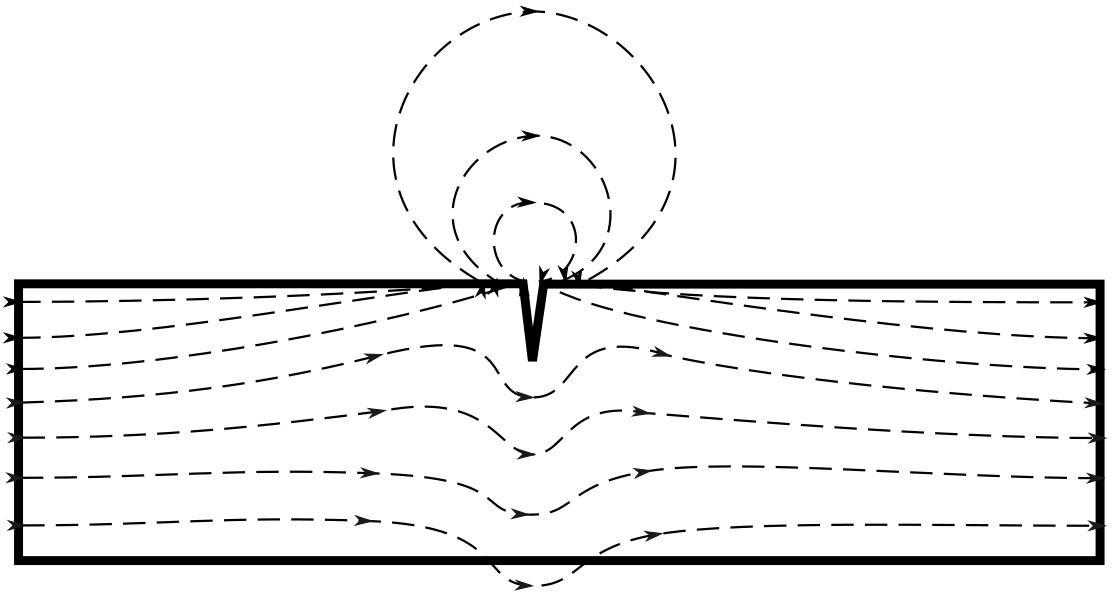
\includegraphics[width=0.75\textwidth]{./Figures/MMM_dispersion.jpg}
	\caption{Fuga de líneas de flujo magnético asociada a grietas y discontinuidades en la superficie del material.}
	\label{fig:MMM_dispersion}
\end{figure}. 

\section{Caracterización multipolar de una anomalía magnética localizada.}
En el aire la inducción $\vec{B}$ y la excitación $\vec{H}$ son proporcionales: $\vec{B} = \mu_{0}\vec{H}$. En el medio sólido sabemos que: $\vec{B} = \mu_{0}\vec{H} + \vec{M}\;$, siendo $\vec{M}$ la Magnetización\footnote{\url{https://en.wikipedia.org/wiki/Magnetization}}. 

En el caso de ausencia de corrientes podremos plantear que $\vec{\nabla}\times\vec{H} = 0$ y como siempre $\vec{\nabla}\cdot\vec{B} = 0$, entonces resultará que:
\begin{equation}
	\label{eq:mediosLIH6}
	\vec{\nabla}\cdot\vec{H} = -\frac{1}{\mu_{0}}\vec{\nabla}\cdot\vec{M}
\end{equation}
Por lo tanto podremos poner que $\vec{H} = -\vec{\nabla}\varphi_{M}$ siendo $\varphi_{M}(\vec{r})$ un potencial escalar magnético que verifica la ecuación de Poisson:

\begin{equation}
	\label{eq:Poisson}
	\nabla^2\varphi_{M}(\vec{r}) = \frac{1}{\mu_{0}} \nabla \cdot\vec{M}(\vec{r}) 
\end{equation}

La ecuación de Poisson \ref{eq:Poisson} se puede resolver por el método de Gauss-Green \citep{GaussGreen} y la solución resulta de la forma:

\begin{equation}
	\label{eq:GaussGreen}
	\varphi_{M}(\vec{r}) = \frac{1}{4\pi\mu_{0}}\iiint_C \frac{\rho_{M}(\vec{r'})}{\mid\vec{r}-\vec{r'}\mid} \cdot \,dV' + 
	\frac{1}{4\pi\mu_{0}}\iint_{\partial C} \frac{\sigma_{M}(\vec{r'})}{\mid\vec{r}-\vec{r'}\mid} \cdot \,dS'
\end{equation}

Donde la integración se lleva a cabo sobre las componentes primadas $\vec{r'}$ para todo el volumen del sólido  $C$ y su frontera ${\partial C}$ siendo $\rho_{M}$ la densidad volumétrica de magnetización y $\sigma_{M}$ la densidad superficial de magnetización

Como solo nos interesan los apartamientos del campo original del sólido sin anomalías, podemos hacer un desarrollo perturbativo\citep{PerturbationMethod}\citep{SingularPerturbation} de la ecuación \ref{eq:Poisson}:



\begin{equation}
	\label{eq:PoissonPerturbada}
	\nabla^2\delta\varphi_{M}(\vec{r}) = \frac{1}{\mu_{0}} \nabla \cdot\vec{\delta M}(\vec{r}) 
\end{equation}

Dando su solución un desarrollo análogo al de la ecuación \ref{eq:GaussGreen} con los reemplazos correspondientes de:

\begin{equation}
	\label{eq:GaussGreenReemplazos}
	\rho_{M}   \rightarrow \delta\rho_{M},\;\;
	\sigma_{M} \rightarrow \delta\rho_{M},\;\;	  
	C \rightarrow R_{mag}, \;\;	  
	\partial C \rightarrow \partial C \cap R_{mag} = \partial R_{mag}
\end{equation}

Notemos que podrá ser la frontera $\partial C \cap R_{mag}$ vacía si la región de influencia de los defectos significativos no llega hasta la superficie del sólido y el término con $\partial R_{mag}$ desaparecer de \ref{eq:GaussGreen}. Por el contrario si el defecto es justamente una discontinuidad en la superficie del sólido como el indicado en la figura \ref{fig:MMM_dispersion} el vacío sera el conjunto $R_{mag}$ y solo aportara al campo su frontera $\partial R_{mag}$

En el aire próximo a la superficie de la pieza, la perturbación $\delta\rho_{M}$ se puede expresar mediante un desarrollo multipolar respecto de un origen de coordenadas localizado en el interior del defecto $R_{mag}$, de modo que el vector posición $\vec{r}$ del punto donde se considera el campo posea un módulo $r$ mayor que el de cualquier vector posición $\vec{r'}$ correspondientes a los puntos donde $\delta \vec{M}(\vec{r'}) \neq 0$. La expresión del desarrollo multipolar correspondiente quedará como:

\begin{equation}
	\label{eq:DesarrolloMultipolar}
	\delta\varphi_{M} \approx \delta\varphi_{M dipolar} + \delta\varphi_{M cuadrupolar} + . . . + . . . 
\end{equation}

Puesto que no existen monopolos magnéticos el desarrollo comenzará con el término dipolar $\delta\vec{\lambda}$ caracterizado por tres componentes de momento dipolar independientes:

\begin{equation}
	\label{eq:Dipolo}
	\delta\vec{\lambda} = \iiint_{R_{mag}} \delta\rho_{M}\; \vec{r'} \,dV' + 
	\iint_{\partial R_{mag}} \delta\sigma_{M}\;  \vec{r'} \,dS'
\end{equation}

Siendo el término correspondiente en el desarrollo multipolar: 

\begin{equation}
	\label{eq:GaussGreenDipolo}
	\delta\varphi_{M}(\vec{r})_{dipolar} \approx \frac{1}{4\pi\mu_{0}} \frac{\delta\vec{\lambda} \cdot \vec{r}}{r^3}
	, \;\;\;\; \mid \vec{r} \mid \gg \mid \vec{r'} \mid 
\end{equation}



El siguiente término, correspondiente al momento cuadrupolar viene caracterizado por cinco coeficientes de cuadrupolo independientes:

\begin{equation}
	\label{eq:Cuadrupolo}
	\delta Q_{ij} = \iiint_{R_{mag}} \delta\rho_{M}\;  \left( 3 x'_{i}x'_{j}-r'^2 \delta_{ij} \right) \,dV' + 
	\iint_{\partial R_{mag}} \delta\sigma_{M}\;  \left( 3 x'_{i}x'_{j}-r'^2 \delta_{ij} \right) \,dS'
\end{equation}

donde $\delta_{ij}$ representa la función delta de Kronecker \footnote{\url{https://en.wikipedia.org/wiki/Kronecker\_delta}}. Observemos que aunque $\delta Q_{ij}$ tiene nueve componentes de su definición resulta que es simétrico y de traza nula \textit{i.e.} $Q_{kl}=Q_{lk}$ y $Q_{11}+Q_{22}+Q_{33}=0 $ razones éstas por lo que solo habrá cinco componentes independientes.

Quedando el término correspondiente en el desarrollo multipolar: 

\begin{equation}
	\label{eq:GaussGreenCuadrupolo}
	\delta\varphi_{M}(\vec{r})_{cuadrupolo} \approx 
	\frac{1}{4\pi\mu_{0}} 
	\frac{\vec{r} \cdot \delta\hat{Q} \cdot \vec{r}}{r^5}
\end{equation}

Fuera del sólido los términos cuadrupolares, octpolares y demás siguientes en la serie tienen  un rápido decaimiento debido a la fuerte dependencia con $\frac{1}{r^{2n+1}}$ para $n \geq 3, 4, ... $. siendo su aporte al campo $\delta\vec{H}$ de segundo orden con respecto al del dipolo. Por lo tanto considerando la perturbación a primer orden, sólo serán relevantes los términos dipolares. Recordemos que estamos hablando de la perturbación $\delta\vec{H}$ y no del campo base $\vec{H}$.     

Tendremos entonces que: la perturbación $\delta\vec{H}$ a primer orden del campo excitación $\vec{H}$ en las proximidades de la superficie del sólido debido a la presencia de un defecto en la región $R_{mag}$ será:

\begin{equation}
	\label{eq:GaussGreenFinal}
	\delta\vec{H}(\vec{r}) = -\nabla\delta\varphi_{M} \approx \frac{1}{4\pi\mu_{0}}\left(  
	\frac{-\delta\vec{\lambda}}{{\mid\vec{r}-\vec{r_{d}}\mid}^3} + 
	\frac{	\left( \delta\vec{\lambda} \cdot \left( \vec{r}-\vec{r_{d}} \right) \right) }{ {\mid\vec{r}-\vec{r_{d}}\mid}^5} 
	\left( \vec{r}-\vec{r_{d}} \right) \right) 
\end{equation}


Siendo $\vec{r_{d}}$ la posición del dipolo $\vec{\lambda}$ respecto de un origen externo de coordenadas fijado arbitrariamente .

A partir de mediciones de $\delta\vec{H}(\vec{r_{k}}) $ se pueden estimar la posición $\vec{r_{d}}$ y las componentes de $\delta\vec\lambda$ aplicando modelos de regresión no lineal\citep{EstimacionNoLineal1}, pudiendo emplearse el algoritmo de Gauss-Newton\footnote{\url{https://en.wikipedia.org/wiki/Gauss-Newton\_algorithm}} cuando se trata de defectos bien localizados como en el caso de fisuras superficiales o próximas a la superficie del sólido . 


De ser necesario continuar a segundo orden con las componentes del desarrollo cuadrupolar, luego de determinarse $\vec{r_{d}}$ y $\delta\vec\lambda$ éstas se eliminarían como incógnitas de la ecuación \ref{eq:GaussGreenFinal} y se le sumaría el término correspondiente al cuadrupolo: 

\begin{equation}
	\label{eq:GaussGreenCuadrupoloFinal}
	-\nabla\delta\varphi_{M}(\vec{r})_{cuadrupolo} \approx 
	-\nabla \left( \frac{1}{4\pi\mu_{0}} 
	\frac{\vec{r} \cdot \delta\hat{Q} \cdot \vec{r}}{r^5}\right) 
\end{equation}

Los cinco coeficientes cuadrupolares incógnita ahora podrán calcularse tomando una nueva serie de mediciones $\delta\vec{H}(\vec(r_{k}) $ y aplicando nuevamente un modelo de regresión no lineal. Para esta forma de funciones en particular resulta apropiado el modelo de Levenberg-Marquardt \citep{EstimacionNoLineal2}. éste modelo es más robusto que el de Gauss-Newton y resulta muy útil cuando no se tiene bien establecida una zona de confianza\footnote{\url{https://en.wikipedia.org/wiki/Levenberg-Marquardt\_algorithm}}.



